\documentclass[11pt, dvipsnames, handout]{beamer}
\newtoggle{full}
\settoggle{full}{true}

\newtoggle{covered}
\settoggle{covered}{false}

\newtoggle{presentable}
\settoggle{presentable}{false}

\newtoggle{dualscreen}
\settoggle{dualscreen}{false}

\usepackage{pgfplots}
%\pgfplotsset{compat = newest}

\usepackage{pgfpages}

\setbeamertemplate{note page}{\pagecolor{yellow!5}\vfill \insertnote \vfill}
\usepackage{collect}
\definecollection{notes}
\newcounter{notestaken}

\usepackage{xpatch}

\usepackage{ulem}

\usepackage[framemethod=tikz]{mdframed}

\usepackage{scalerel}
\usepackage{calc}

%\usepackage{enumitem}
\setlength\fboxsep{.2em}

\usepackage{graphicx} % Allows including images
\usepackage{booktabs} % Allows the use of \toprule, \midrule and \bottomrule in tables

\xpatchcmd{\itemize}
  {\def\makelabel}
  {\setlength{\itemsep}{0.65 em}\def\makelabel}
  {}
  {}


\xpatchcmd{\beamer@enum@}
  {\def\makelabel}
  {\setlength{\itemsep}{0.65 em}\def\makelabel}
  {}
  {}


%\makeatletter
%\renewcommand{\itemize}[1][]{%
%  \beamer@ifempty{#1}{}{\def\beamer@defaultospec{#1}}%
%  \ifnum \@itemdepth >2\relax\@toodeep\else
%    \advance\@itemdepth\@ne
%    \beamer@computepref\@itemdepth% sets \beameritemnestingprefix
%    \usebeamerfont{itemize/enumerate \beameritemnestingprefix body}%
%    \usebeamercolor[fg]{itemize/enumerate \beameritemnestingprefix body}%
%    \usebeamertemplate{itemize/enumerate \beameritemnestingprefix body begin}%
%    \list
%      {\usebeamertemplate{itemize \beameritemnestingprefix item}}
%      {%
%        \setlength\topsep{1em}%NEW
%        \setlength\partopsep{1em}%NEW
%        \setlength\itemsep{1em}%NEW
%        \def\makelabel##1{%
%          {%
%            \hss\llap{{%
%                \usebeamerfont*{itemize \beameritemnestingprefix item}%
%                \usebeamercolor[fg]{itemize \beameritemnestingprefix item}##1}}%
%          }%
%        }%
%      }
%  \fi%
%  \beamer@cramped%
%  \raggedright%
%  \beamer@firstlineitemizeunskip%
%}
%
%
%
%
%
%\makeatother

%\setlist[beamer@enum@]{topsep=1 em}
%\let\origcheckmark\checkmark %screw you dingbat
%\let\checkmark\undefined %screw you dingbat
%\usepackage{dingbat} 
%\let\checkmark\origcheckmark %screw you dingbat






%\usepackage{fontawesome}

\usepackage{mathtools}
\usepackage{etoolbox, calculator}

\usepackage{xcolor}
\usepackage{tikz}
\usetikzlibrary{arrows.meta}
\usetikzlibrary{calc}
\usepackage[nomessages]{fp}
\usepackage{transparent}
\usepackage{accsupp}
%\usepackage{color, xcolor}

%colorblind-friendly palette
%\definecolor{dblue}{RGB}{51,34,136}
\definecolor{lblue}{RGB}{136,204,238}
%\definecolor{green}{RGB}{17,119,51}
\definecolor{tan}{RGB}{221,204,119}
%\definecolor{mauve}{RGB}{204,102,119}

\usepackage{tcolorbox}



\usepackage{xifthen}
\usepackage{nicefrac}
\usepackage{amsmath}
\usepackage{amsthm}
\usepackage{amssymb}
\theoremstyle{definition}
\newtheorem*{define}{Definition}
\newtheorem*{recall}{Recall}


\DeclareMathOperator{\tr}{tr}

\usepackage{multicol}
%\setlength{\columnsep}{1cm}

\usepackage{tablists, amsmath,vwcol, cancel, polynom}
\usetikzlibrary{shapes, patterns, decorations.shapes}
%\usepackage{tikzpeople}
\tikzstyle{vertex}=[shape=circle, minimum size=2mm, inner sep=0, fill]
\tikzstyle{opendot}=[shape=circle, minimum size=2mm, inner sep=0, fill=white, draw]

% common math quick commands
\newcommand{\nicedd}[2]{\nicefrac{\text{d}#1}{\text{d}#2}}
\newcommand{\dd}[2]{\dfrac{\text{d}#1}{\text{d}#2}}
\newcommand{\pd}[2]{\dfrac{\partial #1}{\partial#2}}
\renewcommand{\d}[1]{\text{d}#1}
\newcommand{\ddn}[3]{\dfrac{\text{d}^{#3}#1}{\text{d}#2^{#3}}}
\newcommand{\pdn}[3]{\dfrac{\partial^{#3}#1}{\partial#2^{#3}}}
\newcommand{\p}[0]{^{\prime}}
\newcommand{\pp}[0]{^{\prime\prime}}
\newcommand{\op}[2][\text{L}]{#1 \left[ #2 \right]}

\newcommand{\lap}[1]{\mathcal{L}\left\{#1\right\}}
\newcommand{\lapinv}[1]{\mathcal{L}^{-1}\left\{#1\right\}}
\newcommand{\lapint}[1]{\int_0^\infty e^{-st}#1dt}
\newcommand{\evalat}[2]{\Big|_{#1}^{#2}}

\newcommand{\paren}[1]{ \left( #1 \right)}

\newcommand{\haxis}[4][\normcolor]{\draw[#1, <->] (-#2,0)--(#3,0) node[right]{$#4$}; }


\newcommand{\axis}[4]{\draw[\normcolor, <->] (-#1,0)--(#2,0) 
node[right]{$x$};
\draw[help lines, <->] (0,-#3)--(0,#4) node[above]{$y$};}

\newcommand{\laxis}[6]{\draw[<->] (-#1,0)--(#2,0) 
node[right]{$#5$};
\draw[ <->] (0,-#3)--(0,#4) node[above]{$#6$};}
\newcommand{\xcoord}[2]{
	\draw (#1,.2)--(#1,-.2) node[below]{$#2$};}
\newcommand{\textnode}[3]{
	\draw (#1,#2) node[below]{$#3$};}
	
\newcommand{\nxcoord}[2]{
	\draw (#1,-.2)--(#1,.2) node[above]{$#2$};}
\newcommand{\ycoord}[2]{
	\draw (.2,#1)--(-.2,#1) node[left]{$#2$};}
\newcommand{\nycoord}[2]{
	\draw (-.2,#1)--(.2,#1) node[right]{$#2$};}
\newcommand{\dlim}{\displaystyle\lim}
\newcommand{\dlimx}[1]{\displaystyle\lim_{x \rightarrow #1}}
\newcommand{\stickfig}[2]{
	\draw (#1,#2) arc(-90:270:2mm);
	\draw (#1,#2)--(#1,#2-.5) (#1-.25,#2-.75)--(#1,#2-.5)--(#1+.25,#2-.75) (#1-.2,#2-.2)--(#1+.2,#2-.2);}	

%\newcounter{example}
%\setcounter{example}{1}
%\newcounter{preFrameExample}
%\AtBeginEnvironment{frame}{\setcounter{preFrameExample}{\value{example}}}
%\newcommand{\ex}[1]{
%	 \setcounter{example}{\value{preFrameExample}}
%	 \textcolor{green}{\small\fbox{Example \arabic{example}: #1}}\\[8pt]
%	\stepcounter{example}}
%\newcommand{\exans}[1]{
%	\SUBTRACT{\value{preFrameExample}}{1}{\n}
%	 \textcolor{green}{\small\fbox{Solution \n: #1}}\\[8pt]}
\mode<presentation> {

% The Beamer class comes with a number of default slide themes
% which change the colors and layouts of slides. Below this is a list
% of all the themes, uncomment each in turn to see what they look like.


\usetheme{CambridgeUS}
\usecolortheme[named=black]{structure}


\newcommand{\studentcolor}[0]{ForestGreen}
\newcommand{\normcolor}[0]{NavyBlue}
\newcommand{\alertcolor}{Red}

\setbeamercolor{normal text}{fg=\normcolor}
\setbeamercolor{frametitle}{fg=\normcolor}
\setbeamercolor{section in head/foot}{fg=Black, bg=Gray!20}
\setbeamercolor{subsection in head/foot}{fg=Green!70!Black, bg=Gray!10}
\setbeamercolor{alerted text}{fg=\alertcolor}
\setbeamerfont{alerted text}{series=\bf}
\setbeamertemplate{enumerate items}[default]
\setbeamercolor{enumerate item}{fg=\normcolor}

\setbeamertemplate{footline} % To remove the footer line in all slides uncomment this line
%\setbeamertemplate{footline}[page number] % To replace the footer line in all slides with a simple slide count uncomment this line

\setbeamertemplate{navigation symbols}{} % To remove the navigation symbols from the bottom of all slides uncomment this line
}

\newcommand{\alertbox}[1]{\tcbox[on line, colframe=\alertcolor, colback=White, left=2pt,right=2pt,top=2pt,bottom=2pt]{\usebeamercolor*{normal text}#1}}


\newcommand{\startstu}{\setbeamercolor{normal text}{fg=\studentcolor}\usebeamercolor*{normal text}\setbeamercolor{enumerate item}{fg=\studentcolor}\usebeamercolor*{enumerate item}}
\newcommand{\stopstu}{\setbeamercolor{normal text}{fg=\normcolor}\usebeamercolor*{normal text}\setbeamercolor{enumerate item}{fg=\normcolor}\usebeamercolor*{enumerate item}}

\newcommand{\takenote}[1]{ \begin{collect}{notes}{}{}{}{}  #1  \end{collect}  \addtocounter{notestaken}{1}} %\ifthenelse{\value{notestaken}>0}{\hrulefill\\}{}

\makeatletter
\newcommand{\cover}{\alt{\beamer@makecovered}{\beamer@fakeinvisible}}
\newcommand{\ucover}[1]{\iftoggle{full}{}{\beamer@endcovered}\stopstu#1\startstu\iftoggle{full}{}{\beamer@startcovered}}
\makeatother

\newcommand{\skippause}{ \addtocounter{beamerpauses}{-1}}
\newcommand{\blockpres}{ \skippause \pause }

\newcommand{\studentify}[1]{\startstu #1  \stopstu }
\newcommand{\student}[1]{\iftoggle{full}{ \pause  \studentify{#1} }{\iftoggle{covered}{\studentify{#1}}{\cover{  #1 }}}}
\newcommand{\cstudent}[1]{\student{\begin{center} #1 \end{center}}}
\newcommand{\fullonly}[1]{\iftoggle{full}{ #1}{}}
\newcommand{\presentonly}[1]{\iftoggle{presentable}{ #1}{}}

\usepackage{xparse}
\usepackage{xifthen}

% shortcuts for commonly-used presentation elements
%\NewDocumentCommand{\slide}{o m}
% {\IfValueTF{#1}{\begin{frame}[t]{#1}}{\begin{frame}[t]} #2 \end{frame}}

\newtoggle{iscovered}

\newcommand{\slide}[2][]{%
%\setcounter{notestaken}{0}
\takenote{#2} 
%\ifthenelse{\equal{#1}{}}{\begin{frame}[t]}{\begin{frame}[t]{#1}} #2 \ifthenelse{\value{notestaken}>0}{ \note{\includecollection{notes}}}{} \end{frame}%
\ifthenelse{\equal{#1}{}}{\begin{frame}[t]}{\begin{frame}[t]{#1}} #2 \iftoggle{covered}{\settoggle{iscovered}{true}}{\settoggle{iscovered}{false}}  \note{ \iftoggle{iscovered}{}{\settoggle{covered}{true}} #2 \iftoggle{iscovered}{}{\settoggle{covered}{false}} } \end{frame}%
%\setcounter{notestaken}{0}
}
\newcommand{\defn}[2][]{%
 \setcounter{listcounter}{0}%
\ifthenelse{\equal{#1}{}}{\begin{block}{Definition}}{\begin{block}{#1 :}}%
 #2 \vspace{0.25em} \ifthenelse{\value{listcounter}>0}{\skippause}{} \pause \end{block}%
}



\newcommand{\arr}[2]{\begin{array}{#1}#2\end{array}}
\newcommand{\mat}[2]{\left[\arr{#1}{#2}\right]}
\newcommand{\carray}[1]{\arr{c}{#1}}
\newcommand{\larray}[1]{\arr{l}{#1}}
\newcommand{\rarray}[1]{\arr{r}{#1}}
\newcommand{\colvec}[1]{\mat{c}{#1}}

\newcommand{\itmz}[1]{\addtocounter{listcounter}{1} \begin{itemize}#1 \end{itemize} }
\newcommand{\subitem}[1]{\addtocounter{listcounter}{1} \begin{itemize} \item #1 \end{itemize}}
%
\newcommand{\enum}[1]{\addtocounter{listcounter}{1} \begin{enumerate} #1  \end{enumerate}  }


\newcommand{\algnlbl}[1]{\begin{align}#1  \end{align}} 
\newcommand{\algn}[1]{\begin{align*}#1  \end{align*}} 
\newcommand{\lgn}[1]{ \action<+->{#1} }
\newcommand{\slgn}[1]{\iftoggle{full}{\action<+->{ \startstu #1 \stopstu}}{ \cover{ #1 } } \takenote{$#1$}}

\newcommand{\chckmrk}{\alert{\checkmark}}

\usepackage{pifont}
\newcommand{\xmark}{\alert{\text{\large \ding{55}}}}

\newcommand{\return}[0]{\raisebox{.5ex}{\rotatebox[origin=c]{180}{$\Lsh$}}}
\usepackage{pbox}
%\newcommand{\ex}[1]{\rotatebox[origin=c]{10}{\uline{ex}}:$\;$\pbox[t][][b]{0.9\linewidth}{#1}}
\newcommand{\ex}[1]{\uline{ex}:$\;$\pbox[t][][t]{0.9\linewidth}{#1}}
\newcommand{\eg}[1]{e.g.,$\;$\pbox[t][][t]{0.9\linewidth}{#1}}
\newcommand{\tikzplot}[8][]{%
\begin{tikzpicture}

\begin{scope}[]%
\clip(-#2,-#4) rectangle (#3,#5);%
#8%
\end{scope}%
\laxis{#2}{#3}{#4}{#5}{#6}{#7}%
#1
\end{tikzpicture}%
}


\newcommand{\cancelslide}[1]{%
\begingroup%
\setbeamertemplate{background canvas}{%
\begin{tikzpicture}[remember picture,overlay]%
\draw[line width=2pt,red!60!black] %
  (current page.north west) -- (current page.south east);%
\draw[line width=2pt,red!60!black] %
  (current page.south west) -- (current page.north east);%
\end{tikzpicture}}%
#1%
\endgroup%
}
\renewcommand{\CancelColor}{\color{red}}
\newcommand{\twocols}[3][0.5]{\begin{columns}\begin{column}{#1\textwidth}#2\end{column}\hspace{1em}\vrule{}\hspace{1em}\begin{column}{#1\textwidth}#3\end{column}\end{columns}}

\newcommand{\twomini}[5][1]{\calculatespace \begin{minipage}[t]{\columnwidth}\begin{minipage}[][#1\contentheight][t]{#2\columnwidth}#4\end{minipage}\hfill\begin{minipage}[][#1\contentheight][t]{#3\columnwidth}#5\end{minipage}\end{minipage}}

\newcommand{\threemini}[7][1]{\calculatespace \begin{minipage}[t]{\columnwidth}\begin{minipage}[][#1\contentheight][t]{#2\columnwidth}#5\end{minipage}\hfill\begin{minipage}[][#1\contentheight][t]{#4\columnwidth}#6\end{minipage}\hfill\begin{minipage}[][#1\contentheight][t]{#3\columnwidth}#7\end{minipage}\end{minipage}}


\newcounter{listcounter}
\setcounter{listcounter}{0}



\newif\ifsidebartheme
\sidebarthemetrue

\newdimen\contentheight
\newdimen\contentwidth
\newdimen\contentleft
\newdimen\contentbottom
\makeatletter
\newcommand*{\calculatespace}{%
\contentheight=\paperheight%
\ifx\beamer@frametitle\@empty%
    \setbox\@tempboxa=\box\voidb@x%
  \else%
    \setbox\@tempboxa=\vbox{%
      \vbox{}%
      {\parskip0pt\usebeamertemplate***{frametitle}}%
    }%
    \ifsidebartheme%
      \advance\contentheight by-1em%
    \fi%
  \fi%
\advance\contentheight by-\ht\@tempboxa%
\advance\contentheight by-\dp\@tempboxa%
\advance\contentheight by-\beamer@frametopskip%
\ifbeamer@plainframe%
\contentbottom=0pt%
\else%
\advance\contentheight by-\headheight%
\advance\contentheight by\headdp%
\advance\contentheight by-\footheight%
\advance\contentheight by4pt%
\contentbottom=\footheight%
\advance\contentbottom by-4pt%
\fi%
\contentwidth=\paperwidth%
\ifbeamer@plainframe%
\contentleft=0pt%
\else%
\advance\contentwidth by-\beamer@rightsidebar%
\advance\contentwidth by-\beamer@leftsidebar\relax%
\contentleft=\beamer@leftsidebar%
\fi%
}
\makeatother


\iftoggle{dualscreen}{\setbeameroption{show notes on second screen=right}}{}

\usepackage{gensymb}
\begin{document}
\section{Lecture 31}\subsection{Dirichlet problems continued}
\slide[Dirichlet Problem - with a derivative]{
\ex{Consider a rectangular region of width $w$ and height $h$.}

\vfill
Boundary values are zero at three of the four edges, and the derivative of $u$ obeys some arbitrary function $f(x)$ the fourth edge.\vfill
\twomini[.4]{.5}{.5}{\algn{\Delta u &=0 \\
u(0,y)&=0 &\text{for } 0<y<h\\
u(x,h)&=0 &\text{for } 0<x<w\\
u(w,y)&=0 &\text{for } 0<y<h\\
u_y(x,0)&=f(x) &\text{for } 0<x<w }}{\vspace{.5cm} \centerline{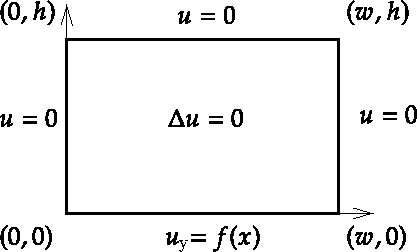
\includegraphics[width=.85\columnwidth]{images/dirichsetup_south_derivative.pdf}}}

}



\slide{\vspace{-2em}
\[ u_{xx}+u_{yy} = 0 \]
Separation of Variables: \[u(x,y) = X(x)Y(y)\]\vspace{-2em}
\student{\algn{X\pp Y+XY\pp &= 0 \\
\frac{X\pp(x)}{X(x)} = -\frac{Y\pp(y)}{Y(y)} &= -\lambda = \text{const.}}\vfill
\twomini[.15]{.5}{.5}{\[X\pp+\lambda X =0 \]}{\[Y\pp-\lambda Y =0 \]



}
BCs: $X(0)=X(w)=0$

\[X_n(x)= \sin \left( \frac{n\pi}{w} x \right)  \qquad \lambda_n = \left(\frac{n\pi}{w}\right)^2\]
}
}


\slide{
\twomini[.35]{.5}{.45}{\[Y\pp-\lambda Y =0 \] \vfill\[ \lambda = \left(\frac{n\pi}{w}\right)^2\] \vfill }{ \centerline{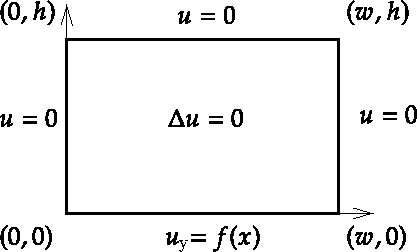
\includegraphics[width=.85\columnwidth]{images/dirichsetup_south_derivative.pdf}} }
\vfill
So far, this is exactly what we had solving the south problem
\vfill
\student{
\[u_{n}(x,y) = a_n \sin \left( \frac{n\pi}{w}x \right) \sinh \left( \frac{n\pi}{w} (h-y)\right) \qquad u(x,y)=\sum_n u_n\]
\[f(x) = \sum_n b_n \cos\left( \frac{n\pi}{w} x \right) = u_y(x,0) \]
\[u_y(x,0) = \sum_n a_n  \frac{n\pi}{w}\cosh \left( \frac{n\pi}{w} h\right) \sin \left( \frac{n\pi}{w}x \right)  \qquad \boxed{ a_n = \frac{b_n}{\cosh\left( \frac{n\pi}{w} \right) } \frac{w}{n\pi}} \]
}
}

\slide{
\ex{Consider the following problem}


\twomini[.4]{.5}{.5}{\algn{\Delta u &=0 \\
u(0,y)&=2 &\text{for } 0<y<1\\
u(x,h)&=0 &\text{for } 0<x<2\\
u(2,y)&=3 \sin(\pi y) &\text{for } 0<y<1\\
u_y(x,0)&=x(1-x) &\text{for } 0<x<2 }}{\vspace{.5cm} \centerline{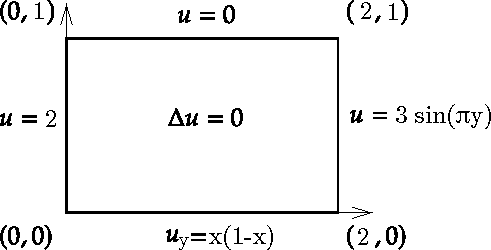
\includegraphics[width=.85\columnwidth]{images/dirichsetup_ex2.pdf}}}\vfill
\student{
Strategy: Break the problem down into West, East, and South Problems, then use superposition.
\[u(x,y) =u_W +u_E+u_S\]
}
}

\slide{
\student{West problem
\[u_W(x,y) = \sum_n d_n \sin \left( n\pi y \right) \sinh \left( n\pi (2-x)\right)\]
\[u_W(0,y) = 2 = \sum_n d_n \sin \left( n \pi y \right) \sinh \left(  2 n\pi\right)\]
\[2=\sum_n b_n \sin \left( n\pi y \right)  \qquad b_n=\frac{2}{1} \int_0^1 2 \sin(n \pi y)dy = 4\frac{1-(-1)^n}{n\pi}    \]
\[d_n = \frac{b_n}{\sinh(2n\pi)}  = 4\frac{1-(-1)^n}{\sinh(2n\pi)n\pi}  \]
}
}

\slide{
\student{East problem
\[u_E(x,y) = \sum_n c_n \sin \left( n\pi y \right) \sinh \left(n\pi x\right) \]
\[u_E(2,y) = 3sin(\pi y) = \sum_n c_n \sin \left( n \pi y \right) \sinh \left(  2 n\pi\right)\]
\[3sin(\pi y)=\sum_n b_n \sin \left( n\pi y \right)  \qquad b_n=\begin{cases} 3 & n=1\\0&\text{otherwise} \end{cases}  \]
\[c_n = \frac{b_n}{\sinh(2n\pi)}  = \begin{cases} \frac{3}{\sinh(2\pi)} & n=1\\0&\text{otherwise} \end{cases} \]
}
}

\slide{
\student{South problem
\[u_S(x,y) =  \sum_n a_n \sin \left( \frac{n\pi}{2} x \right) \sinh \left( \frac{n\pi}{2} (1-y)\right) \]
\[\pd{}{y} u_S(x,0) = x(1-x)= \sum_n a_n \sin \left(\frac{n\pi}{2} x \right) \frac{n\pi}{2} \cosh \left( \frac{n\pi}{2} \right) \]
\[x(1-x)=\sum_n b_n \sin \left( \frac{n\pi}{2} x \right)  \qquad \boxed{ a_n =- \frac{2}{n\pi}\frac{b_n}{ \cosh\left(\frac{n\pi}{2}\right)} }\]
\[ b_n= \frac{2}{2} \int_0^2 x(1-x) \sin \left(\frac{n\pi}{2} x \right)  dx = \frac{4 (-1)^n \left(\pi ^2 n^2-4\right)+16}{\pi ^3 n^3} \]

\vfill
Finally, 
\[u(x,y) =u_W +u_E+u_S\]
}
}
\subsection{Neumann Problems}
\slide[Derivatives in higher dimensions]{
For $u=u(x,y)$, we can compute two derivatives along the coordinate axes\student{ \algn{u_x &= \pd{}{x}u(x,y) \\u_y &= \pd{}{y}u(x,y)}}
\vfill
The generalization of this is a directional derivative (or gradient) $\vec{\nabla}u$\vfill
\student{\[\vec{\nabla}u =\underbrace{ \mat{c}{u_x \\ u_y}}_{\text{vector}}\]}\vfill
}

\slide[Neumann Boundary Conditions]{
Consider $\vec{x}\in\mathbb{R}^d$ restricted to a closed domain, where the boundary of the domain has a outer unit normal vector $\hat{n}$.
\vfill
\centerline{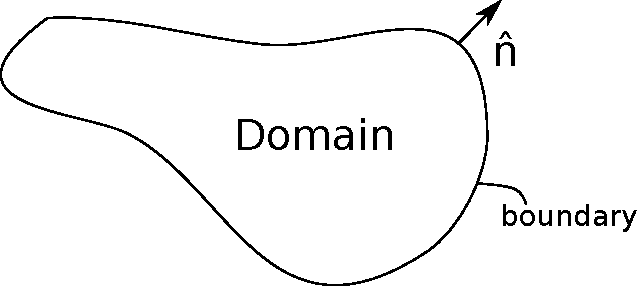
\includegraphics[width=6cm]{images/generic_domain.pdf}}
\vfill
The Neumann boundary condition is given by \[\pd{u}{\hat{n}} = f(\vec{x})  \qquad\text{ for $\vec{x}$ along the boundary}  \]$\pd{u}{\hat{n}} = \vec{\nabla}u\cdot\hat{n}$
}

\slide[Neumann Boundary Condition Example - Electrostatics]{
Consider Maxwell's 1st equation \[\vec{\nabla}\cdot \vec{E}(x,y) = \frac{\rho}{\varepsilon_0} = \frac{\text{charge density}}{\text{permittivity of free space}}\]applied to a charged 2D box with with charge density $\rho_0$ that sits in an external electric field
$\vec{E}_{ext}=\vec{E}_{ext}(x,y)$.

\vfill

\twomini[.45]{.65}{.35}{
The electric field is the negative gradient of the electric potential $u(x,y)$\student{ \[\vec{E} =- \vec{\nabla}u \]
\[\Rightarrow \vec{\nabla} \cdot \vec{E} = - \nabla^2 u = - \Delta u \]
\[\Rightarrow  - \Delta u =\frac{\rho}{\varepsilon_0}\]
}
}{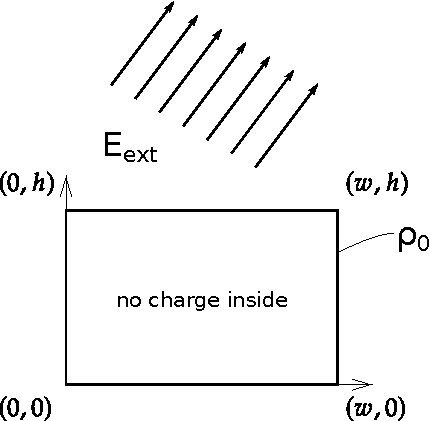
\includegraphics[width=\columnwidth]{images/electrostatic_neumann_setup.pdf}}

}

\slide[Neumann Boundary Condition Example - Electrostatics]{

\twomini[.65]{.65}{.35}{

\[\Delta u = 0 \qquad  \text{for $(x,y)$ inside the box}\]
Boundary Conditions:
\small
\[-\pd{u}{\hat{n}} - \vec{E}_{ext}(x,t) \cdot \hat{n} = \frac{\rho_0}{\varepsilon_0}\]
\student{North side:
\algn{-\left(u_x\hat{i} + u_y \hat{j}\right) \cdot \hat{j} &= \frac{\rho_0}{\varepsilon_0}+\vec{E}_{ext}(x,h)\cdot\hat{j}\\
u_y(x,h) &=f(x)}
}
\algn{}}{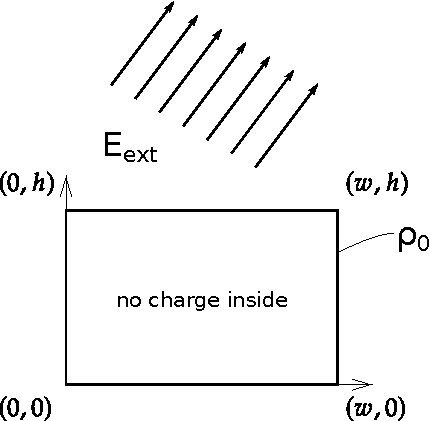
\includegraphics[width=\columnwidth]{images/electrostatic_neumann_setup.pdf}}

\small
\student{West Side:
\algn{-\left(u_x\hat{i} + u_y \hat{j}\right) \cdot -\hat{i} &= \frac{\rho_0}{\varepsilon_0}+\vec{E}_{ext}(0,y)\cdot-\hat{i}\\
u_x(0,y) &=g(x)}
}


}


\subsection{Neumann problems}
\slide[Neumann Problem]{
\ex{Consider a rectangular region of width $w$ and height $h$.}

\vfill
Normal derivatives are zero at three of the four edges, and the derivative of $u$ obeys some arbitrary function $f(x)$ the fourth edge.\vfill
\twomini[.4]{.5}{.5}{\algn{\Delta u &=0 \\
u_x(0,y)&=0 &\text{for } 0<y<h\\
u_y(x,h)&=0 &\text{for } 0<x<w\\
u_x(w,y)&=0 &\text{for } 0<y<h\\
u_y(x,0)&=f(x) &\text{for } 0<x<w }}{\vspace{.5cm} \centerline{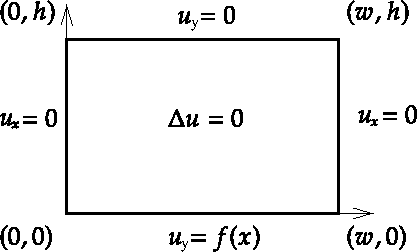
\includegraphics[width=.85\columnwidth]{images/Neumann_setup.pdf}}}

}



\slide{Solution procedure is almost identical to the Dirichlet problem but with $\sin \to \cos $ and $\sinh \to \cosh$\vspace{.25em}
\hrule
\vfill
\twomini[.15]{.5}{.5}{\[X\pp+\lambda X =0 \]}{\[Y\pp-\lambda Y =0 \]
}\vspace{-1em}
BCs: $\pd{}{x}X(0)=\pd{}{x}X(w)=0$
\[X_n(x)= \cos \left( \frac{n\pi}{w} x \right)  \qquad \lambda_n = \left(\frac{n\pi}{w}\right)^2\]\vfill\[\Rightarrow Y_n\pp+\left(\frac{n\pi}{w}\right)^2Y_n=0\qquad \Rightarrow Y_n=Ae^{\frac{n\pi}{w}y}+Be^{-\frac{n\pi}{w}y}\]
BC: $\pd{}{y}Y_n(h)=0$
\[\Rightarrow B=Ae^{2\frac{n\pi}{w}} \qquad \Rightarrow Y_n(y)=a_n \cosh\left( \frac{n\pi}{w} (y-h) \right)  \]
Finally,
\[\boxed{u_n(x,y)=a_n \cosh\left( \frac{n\pi}{w} (y-h) \right) \cos\left(\frac{n\pi}{w} x\right)} \quad u(x,y) = \sum_n u_n(x,y)\]

}

\slide[]{
Major difference with Dirichlet problem: $n=0$ gives a non-zero solution
\student{
\[X_0(x)=\cos(0)=1\]

\[Y_0\pp=0 \Rightarrow Y_0 = m y + a_0\]
$\pd{}{y}Y_0(h)=0=m \qquad \Rightarrow m=0$
\[Y_0 = a_0 \]

\[u(x,y)= a_0+\sum_n a_n \cosh\left( \frac{n\pi}{w} (y-h) \right) \cos\left(\frac{n\pi}{w} x\right) \]
\vfill
Impossible to actually determine $a_0$.\subitem{ e.g., electrical potentials can be shifted arbitrarily}
\vfill
Pure Neumann problems do not have unique solutions.
}
}

\slide[The non-zero boundary condition]{\vspace{-2em}\[u_{n}(x,y) = a_n \cos \left( \frac{n\pi}{w} x \right) \cosh\left( \frac{n\pi}{w} (y-h)\right), \quad u(x,y)=a_0+\sum_{n=1}^{\infty} u_n(x,y)\]\vfill
$u_y(x,0)=f(x) $ - Express the boundary condition as a Fourier Series\vfill
\student{

\algn{u_y(x,0)&=f(x) = a_0+ \sum_{n=1}^{\infty}  a_n \frac{n\pi}{w} \sinh \left( \frac{n\pi}{w} h\right) \cos \left( \frac{n\pi}{w} x \right) \intertext{Given the appearance of our $u_y(x,h)$, we clearly need a Cosine series}
f(x) &=\frac{b_0}{2}+\sum_{n=1}^{\infty} b_n \cos \left( \frac{n\pi}{w} x \right) \qquad \text{with } b_n=\frac{2}{w} \int_0^w f(x) \cos \left( \frac{n\pi}{w} x \right) dx  \\
 \intertext{need equality between the two series}}
\[\Rightarrow b_0 = 0 = \int_0^w f(x) dx \qquad \qquad  a_n = \frac{b_n}{ \sinh \left( \frac{n\pi}{w} h \right)  } \frac{w}{n\pi}\]

}
}


\slide[]{
We can repeat the same process for all the sub-problems.
\vfill
\algn{ u_N &= a_0 + \sum_n a_n \cos \left( \frac{n\pi}{w}x \right) \cosh \left( \frac{n\pi}{w} y\right)\\
u_S &= b_0 + \sum_n b_n \cos \left( \frac{n\pi}{w}x \right) \cosh \left( \frac{n\pi}{w} (h-y)\right)\\
u_E &= c_0 + \sum_n c_n \cos \left( \frac{n\pi}{h}y \right) \cosh \left( \frac{n\pi}{h} x\right)\\
u_W &= d_0 + \sum_n d_n \cos \left( \frac{n\pi}{h} y \right) \cosh \left( \frac{n\pi}{h} (w-x)\right)
}
\vfill
To find the unknow coefficients, match the series solution derivative with a Cosine series of the boundary condition.
\vfill
The boundary condition (normal derivative) must integrate to zero over the boundary.
}


%\slide[Non-Neumann Boundary Conditions]{
%
%\twomini[.4]{.5}{.5}{\algn{\Delta u &=0 \\
%u_x(0,y)&=0 &\text{for } 0<y<h\\
%u_y(x,1)&=0 &\text{for } 0<x<w\\
%u_x(2,y)&=0 &\text{for } 0<y<h\\
%u_x(x,0)&=0 &\text{for } 0<x<w }}{\vspace{.5cm} \centerline{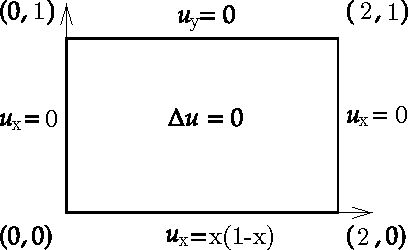
\includegraphics[width=.85\columnwidth]{images/dirichsetup_ex3.pdf}}}
%\student{
%South boundary condition is in
%}
%
%
%}




\slide[Mixed Neumann/Dirichlet Problem]{

\twomini[.4]{.5}{.5}{\algn{\Delta u &=0 \\
u_x(0,y)&=0 &\text{for } 0<y<h\\
u(x,h)&=f(x) &\text{for } 0<x<w\\
u_x(w,y)&=0 &\text{for } 0<y<h\\
u(x,0)&=0 &\text{for } 0<x<w }}{\vspace{.5cm} \centerline{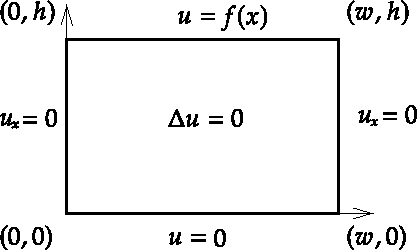
\includegraphics[width=.85\columnwidth]{images/mixed_setup.pdf}}}


}



\slide{\vspace{-2em}
\[ u_{xx}+u_{yy} = 0 \]
Separation of Variables: \[u(x,y) = X(x)Y(y)\]\vspace{-2em}
\student{
\algn{X\pp Y+XY\pp &= 0 \\
\frac{X\pp(x)}{X(x)} = -\frac{Y\pp(y)}{Y(y)} &= -\lambda = \text{const.}}\vfill
\twomini[.15]{.5}{.5}{\[X\pp+\lambda X =0 \]}{\[Y\pp-\lambda Y =0 \]



}
BCs: $X_x(0)=X_x(w)=0$

\[X_n(x)= \cos \left( \frac{n\pi}{w} x \right)  \qquad \lambda_n = \left(\frac{n\pi}{w}\right)^2\]
with the special case $n=0$
\[X_0(x) = 1 \]
}
}

\slide{
\twomini[.35]{.5}{.45}{\[Y\pp-\lambda Y =0 \] \vfill\[ \lambda = \left(\frac{n\pi}{w}\right)^2\] \vfill }{ \centerline{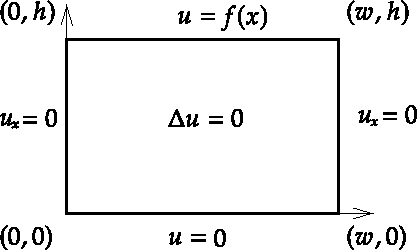
\includegraphics[width=.85\columnwidth]{images/mixed_setup.pdf}} }
\vfill
\vfill
\student{
\uline{$n\neq0$}
\algn{Y_n(y) &= Ae^{\frac{n\pi}{w} y} + B e^{-\frac{n\pi}{w} y}\\
\text{BC @ x=0: } 0&=A+B &\Rightarrow B=-A\\
Y_n(y) &= A \left(e^{\frac{n\pi}{w} y} - e^{-\frac{n\pi}{w} y} \right)\\
&=a_n \sinh\left( \frac{n\pi}{w} y \right)\\
u_n(x,y) &=a_n \sinh\left( \frac{n\pi}{w} y \right) \cos \left( \frac{n\pi}{w} x \right)  
\intertext{\uline{n=0}}
Y_0\pp&=0 \Rightarrow Y_0=a_0y+b\qquad Y_0(0)=0 \Rightarrow b=0
}

}
}

\slide[The non-zero boundary condition]{\vspace{-2em}\[u_{n}(x,y) = a_n \cos \left( \frac{n\pi}{w} x \right) \sinh \left( \frac{n\pi}{w} y\right), \quad u(x,y)=a_0 y +\sum_{n=1}^{\infty} u_n(x,y)\]\vfill
$u(x,h)=f(x) $ - Express the boundary condition as a Fourier Series\vfill
\student{

\algn{u(x,h)&=f(x) = a_0 h + \sum_{n=1}^{\infty}  a_n \sinh \left( \frac{n\pi}{w} h\right) \cos \left( \frac{n\pi}{w} x \right) \intertext{Given the appearance of our $u(x,h)$, we clearly need a Cosine series}
f(x) &=\frac{b_0}{2} + \sum_{n=1}^{\infty} b_n \cos \left( \frac{n\pi}{w} x \right) \qquad \text{with } b_n=\frac{2}{w} \int_0^w f(x) \cos \left( \frac{n\pi}{w} x \right) dx  \\
 \intertext{need equality between the two series}
\Rightarrow a_0&=\frac{b_0}{2h} \qquad \text{and} \qquad  a_n =\frac{b_n}{ \sinh \left( \frac{n\pi}{w} h \right)  } 
}
}
}

\end{document}